\documentclass[11pt]{article}
\usepackage{fullpage}
\usepackage{amsmath,amsthm,amssymb,amsfonts,multirow}
\usepackage{mathtools}
\usepackage{graphicx}
\usepackage{xcolor}
\usepackage{float}
%\usepackage{enumerate}
\usepackage[shortlabels, inline]{enumitem}
\usepackage{textcomp}
\usepackage{hyperref}
\usepackage{comment}

\usepackage{listings}
\lstset{language=Python, numbers=left, basicstyle=\ttfamily, keywordstyle=\color{blue}, showstringspaces=false}

\usepackage[style=alphabetic-verb]{biblatex}
% \bibliography{Problems/ref.bib}

\newcommand{\N}{\mathbb{N}}
\newcommand{\Z}{\mathbb{Z}}
\newcommand{\Q}{\mathbb{Q}}
\newcommand{\R}{\mathbb{R}}
\newcommand{\C}{\mathcal{C}}
\newcommand{\K}{\mathbb{K}}
\renewcommand{\div}{\mid}
\newcommand{\ndiv}{\nmid}
\newcommand{\E}{\mathbb{E}}
\newcommand{\I}{\mathbb{I}}
\newcommand{\F}{\mathcal{F}}

\DeclareMathOperator{\id}{Id}
\DeclareMathOperator{\tr}{Tr}
\DeclareMathOperator*{\argmax}{arg\,max}
\DeclareMathOperator{\lcm}{lcm}
\DeclareMathOperator{\spn}{span}
\DeclareMathOperator{\acosh}{acosh}

\DeclarePairedDelimiter{\floor}{\lfloor}{\rfloor}
\DeclarePairedDelimiter{\ceil}{\lceil}{\rceil}
\DeclarePairedDelimiter{\abs}{\lvert}{\rvert}

\newcommand{\subtag}[1]{\tag{\theparentequation#1}}

\renewcommand{\vec}[1]{\mathbf{#1}}

\usepackage{subfiles}
\usepackage{subcaption}
\makeatletter
\newcommand\nocaption{
    \renewcommand\p@subfigure{}
    \renewcommand{\thesubfigure}{\arabic{figure}\alph{subfigure}}
}
\makeatother


\newenvironment{problem}[2][Question]{\begin{trivlist}
\item[\hskip \labelsep {\bfseries #1}\hskip \labelsep {\bfseries #2.}]}{\end{trivlist}}

\newenvironment{solution}{%
  \begin{proof}[\textbf{Solution}]$ $\par\nobreak\ignorespaces
}{%
  \end{proof}
}

\theoremstyle{definition}
\newtheorem{definition}{Definition}
\newtheorem{theorem}{Theorem}
\newtheorem{lemma}{Lemma}

\hypersetup{
    colorlinks=true,
    linkcolor=blue,
    filecolor=magenta,      
    urlcolor=cyan,
    pdftitle={Overleaf Example},
    pdfpagemode=FullScreen,
    }


\title{Intro to Computational Mathematics: Section 9}
\date{October 2025}

\begin{document}
\maketitle

\begin{problem}{5.2.5}
    Here we consider a proof of \href{https://fncbook.com/pwlin/#theorem-pwlin-converge}{Theorem 5.2.2} using the mean value theorem from elementary calculus: If $f$ is continuously differentiable in $(a, b)$, then there exist points $s$ and $t$ in $(a, b)$ such that $$\int_a^b f(z) \, dz = (b - a)f(s) \qquad \text{and} \qquad f'(t) = \frac{f(b) - f(a)}{b - a}.$$
    For the following, suppose $x \in (t_k, t_{k+1})$.
    \begin{enumerate}[(a)]
        \item Show that for some $s \in (t_k, t_{k+1})$, $$f(x) = y_k + (x - t_k)f'(s).$$
        \item Show that for some other values $u$ and $v$ in $(t_k, t_{k+1})$, $$f'(s) - \frac{y_{k+1} - y_k}{t_{k+1} - t_k} = (s - u)f''(v).$$
        \item Use \href{https://fncbook.com/pwlin/#pwlinear}{(5.2.1)} to finish the proof of the theorem.
    \end{enumerate}
\end{problem}
\begin{solution}
\begin{enumerate}[(a)]
    \item Consider the interval $(t_k, x)$. Since we assume that $f$ has a continuous second derivative in $(a, b)$ it is differentiable in $(t_k, x)$. Thus we have that there exists an $s \in (t_k, x)$ such that:
    \begin{align*}
        f'(s) &= \frac{f(x) - f(t_k)}{x - t_k} \\
        (x - t_k)f'(s) &= f(x) - y_k \\
        f(x) &= y_k + (x - t_k)f'(s)
    \end{align*}
    \item We begin by finding an appropriate choice for $u$. Let $u \in (t_k, t_{k+1})$ be the choice by MVT for which:
    \begin{align*}
        f'(u) = \frac{f(t_{k+1}) - f(t_k)}{t_{k+1} - t_k}
    \end{align*}
    Now since the derivative of $f$ is continuously differentiable, we again use the MVT to find a choice of $v$ in the interval $(u, s)$. (Note that if $u > s$ then the same thing works by multiplying each side by $-1$)
    \begin{align*}
        f''(v) &= \frac{f'(s) - f'(u)}{s - u} \\
        (s - u)f''(v) &= f'(s) - f'(u) \\
        (s - u)f''(v) &= f'(s) - \frac{f(t_{k+1}) - f(t_k)}{t_{k+1} - t_k} \\
        (s - u)f''(v) &= f'(s) - \frac{y_{k+1} - y_k}{t_{k+1} - t_k}
    \end{align*}
    \item We want to find an upper bound for $\|f - p_n\|_\infty = \max_{x \in [a, b]}|f(x) - p(x)|$. We consider this in each interval $[t_k, t_{k+1}]$ separately at first:
    \begin{align*}
        \max_{x \in [t_k, t_{k+1}]}|f(x) - p(x)| &= \max_{x \in [t_k, t_{k+1}]}\left|\left(y_k + (x - t_k)f'(s)\right) - \left(y_k + \frac{y_{k+1} - y_k}{t_{k+1} - t_k}(x - t_k)\right)\right| \\
        &= \max_{x \in [t_k, t_{k+1}]}\left|y_k + (x - t_k)f'(s) - y_k - \frac{y_{k+1} - y_k}{t_{k+1} - t_k}(x - t_k)\right| \\
        &= \max_{x \in [t_k, t_{k+1}]}\left|(x - t_k)f'(s) - \frac{y_{k+1} - y_k}{t_{k+1} - t_k}(x - t_k)\right| \\
        &= \max_{x \in [t_k, t_{k+1}]}\left|(x - t_k)\left(f'(s) - \frac{y_{k+1} - y_k}{t_{k+1} - t_k}\right)\right| \\
        &= \max_{x \in [t_k, t_{k+1}]}\left|(x - t_k)(s - u)f''(v)\right| \\
        &\leq \frac{b - a}{n} \cdot \frac{b - a}{n} \|f''\|_\infty
    \end{align*}
    Since this is true for all segments $[t_k, t_{k+1}]$, we conclude $\|f - p_n\|_\infty \leq Mh^2$ where $h = \frac{b - a}{n}$.
\end{enumerate}
\end{solution}



\begin{problem}{5.3.5}
\begin{enumerate}[(a)]
    \item If $y_0 = y_n$, another possibility for cubic spline end conditions is to make $S(x)$ a periodic function. This implies that $S'$ and $S''$ are also periodic. Write out the two new algebraic equations for these constraints in terms of the piecewise coefficients.
    \item Modify \href{https://fncbook.com/splines/#function-spinterp}{Function 5.3.1} to compute a periodic spline interpolant. Test by making a plot of the interpolant for $f(x) = \exp(\sin(3x))$ over the interval $[0, 2\pi/3]$ with equally spaced nodes and $n = 8$.
\end{enumerate}
\end{problem}
\begin{solution}
\begin{enumerate}[(a)]
    \item The only conditions that change here are the end conditions. Here we automatically pick up the condition that $S(t_0) = S(t_n)$ since $y_0 = y_n$. However, we probably will want our last two conditions to be that $S'(t_0) = S'(t_n)$ and $S''(t_0) = S''(t_n)$.
    \item The following code shows the implementation of this change:
\begin{lstlisting}
import numpy as np
from numpy.linalg import solve
import matplotlib.pyplot as plt

def spinterp(t, y):
    """
    spinterp(t, y)

    Create a cubic not-a-knot spline interpolating function for data values in y given at nodes in t.
    """
    n = len(t) - 1
    h = [t[i + 1] - t[i] for i in range(n)]

    # Preliminary definitions.
    Z = np.zeros([n, n])
    I = np.eye(n)
    E = I[: n - 1, :]
    J = np.eye(n) + np.diag(-np.ones(n - 1), 1)
    J[-1, 0] = -1
    H = np.diag(h)

    # Left endpoint interpolation:
    AL = np.hstack([I, Z, Z, Z])
    vL = y[:-1]

    # Right endpoint interpolation:
    AR = np.hstack([I, H, H**2, H**3])
    vR = y[1:]

    # Continuity of first derivative:
    A1 = np.hstack([Z, J, 2 * H, 3 * H ** 2])
    v1 = np.zeros(n)

    # Continuity of second derivative:
    A2 = np.hstack([Z, Z, J, 3 * H])
    v2 = np.zeros(n)


    # Assemble and solve the full system.
    A = np.vstack([AL, AR, A1, A2])
    v = np.hstack([vL, vR, v1, v2])
    z = solve(A, v)

    # Break the coefficients into separate vectors.
    rows = np.arange(n)
    a = z[rows]
    b = z[n + rows]
    c = z[2 * n + rows]
    d = z[3 * n + rows]
    S = [np.poly1d([d[k], c[k], b[k], a[k]]) for k in range(n)]

    # This function evaluates the spline when called with a value for x.
    def evaluate(x):
        f = np.zeros(x.shape)
        for k in range(n):
            # Evaluate this piece's cubic at the points inside it.
            index = (x >= t[k]) & (x <= t[k + 1])
            f[index] = S[k](x[index] - t[k])
        return f

    return evaluate


def f(x):
    return np.exp(np.sin(3 * x))


t = np.linspace(0, 2*np.pi/3, 8)
f_spline = spinterp(t, [f(t_) for t_ in t])

s = np.linspace(0, 2*np.pi/3, 400)
plt.plot(s, [f_spline(s_) for s_ in s], label='Cubic Spline of f')
plt.plot(s + 2*np.pi/3, [f_spline(s_) for s_ in s], '--', label='Shifted Spline to Show Periodicity')
plt.legend()
plt.title('Periodic Splining')
plt.show()
\end{lstlisting}
Output:
\begin{center}
    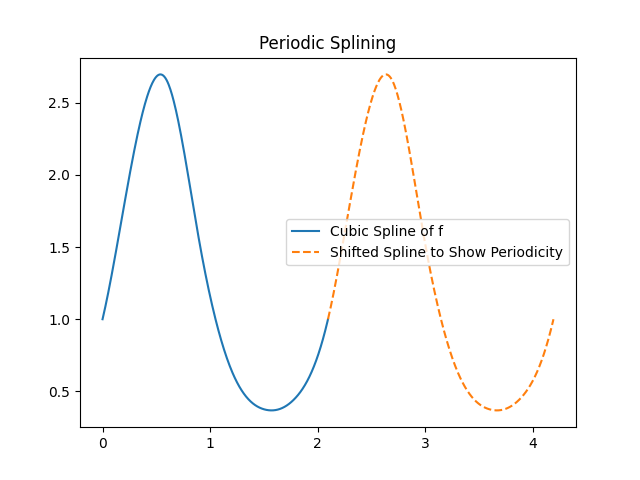
\includegraphics[width=0.8\textwidth]{5.3.5_fig.png}
\end{center}
The only changes that were made to the function \texttt{spinterp} are on lines 19, 31, and 35 respectively. The computations required to compute boundary conditions are already encoded in A1 and A2 respectively as long as we set the last row of $J$ to $[-1, 0, \ldots, 0, 1]$. Since we no longer want to throw these condition lines away, we can remove the left multiplication by $E$ in both lines 31 and 35.
\end{enumerate}
\end{solution}



\begin{problem}{5.4.1}
This problem refers to $Q(x)$ defined by \href{https://fncbook.com/finitediffs/#fdinterp2}{(5.4.4)}.
\begin{enumerate}[(a)]
    \item Show that $Q(x)$ interpolates the three values of $f$ at $x = -h$, $x = 0$, and $x = h$.
    \item Show that $Q'(0)$ gives the finite-difference formula defined by \href{https://fncbook.com/finitediffs/#centerfd12}{(5.4.5)}.
\end{enumerate}
\end{problem}
\begin{solution}
$Q(x) = \frac{x(x - h)}{2h^2}{f(-h)} - \frac{x^2 - h^2}{h^2}f(0) + \frac{x(x+h)}{2h^2}f(h).$
\begin{enumerate}[(a)]
    \item
    \begin{align*}
        Q(-h) &= \frac{(-h)((-h) - h)}{2h^2}{f(-h)} - \frac{(-h)^2 - h^2}{h^2}f(0) + \frac{(-h)((-h)+h)}{2h^2}f(-h) \\
        &= \frac{2h^2}{2h^2}f(-h) - \frac{0}{h^2}f(0) + \frac{0}{2h^2}f(-h) \\
        &= f(-h) \\
        Q(0) &= \frac{0(0 - h)}{2h^2}{f(-h)} - \frac{0^2 - h^2}{h^2}f(0) + \frac{0(0+h)}{2h^2}f(h) \\
        &= f(0) \\
        Q(h) &= \frac{h(h - h)}{2h^2}{f(-h)} - \frac{h^2 - h^2}{h^2}f(0) + \frac{h(h+h)}{2h^2}f(h) \\
        &= \frac{0}{2h^2}f(-h) - 0\frac{0}{h^2}f(0) + \frac{2h^2}{2h^2}f(h) \\
        &= f(h)
    \end{align*}
    \item
    \begin{align*}
        Q'(x) &= \frac{d}{dx}\left[\frac{x(x - h)}{2h^2}{f(-h)} - \frac{x^2 - h^2}{h^2}f(0) + \frac{x(x+h)}{2h^2}f(h)\right] \\
        &= \frac{2x - h}{2h^2}f(-h) - \frac{2x}{h^2}f(0) + \frac{2x + h}{2h^2}f(h) \\
        Q'(0) &= \frac{2(0) - h}{2h^2}f(-h) - \frac{2(0)}{h^2}f(0) + \frac{2(0) + h}{2h^2}f(h) \\
        &= \frac{-h}{2h^2}f(-h) + \frac{h}{2h^2}f(h) \\
        &= \frac{f(h) - f(-h)}{2h}
    \end{align*}
\end{enumerate}
\end{solution}



\begin{problem}{Q2}
Consider the following interpolation problem: For some four times continuously differentiable function $f: [0,1] \rightarrow \R$, let $t_i = i/n$ and $y_i = f(t_i)$ for $i=0\dots n$. Denote the piecewise linear interpolation of the points $(t_i, y_i)$ by $p_n(x)$, the cubic spline interpolation by $q_n(x)$, and the degree $n$ polynomial interpolation by $s_n(x)$.\\

\begin{enumerate}[(a)]
     \item State the definition of the infinity function norm $\|f\|_\infty$.
     \item What orders of convergence (if at all) can we expect the following three quantities are guaranteed to have as $n$ grows: $\|f-p_n\|_\infty$, $\|f-q_n\|_\infty$, and $\|f-s_n\|_\infty$?
     \item For a particular four times differentiable function $f$, numerically computed values for these differences are on the next page. Contrast the observed performance with your claims from (b). Provide a potential explanation for any interesting differences or phenomena you see.


\newpage
\begin{tabular}{| c | l | l | l | }
\hline
$n$ & $\|f-p_n\|_\infty$ & $\|f-q_n\|_\infty$ & $\|f-s_n\|_\infty$ \\ \hline
2 & 1.378559200870535 & 1.2586021146713118 & 1.2007575889406117 \\ 
4 & 0.6646176211627189 & 0.4340726477252055 & 0.08554727877395929 \\ 
6 & 0.3662481666114553 & 0.20630323537691442 & 3.3306690738754696e-15 \\ 
8 & 0.22905150647695494 & 0.11887394189179568 & 4.107825191113079e-15 \\ 
10 & 0.1561326791394949 & 0.07694493400884028 & 1.2101430968414206e-14 \\ 
12 & 0.11305220152975681 & 0.05376679008602603 & 5.162537064506978e-15 \\ 
14 & 0.08556477919265826 & 0.0396514354914515 & 8.79296635503124e-14 \\ 
16 & 0.06698282553600393 & 0.030432940263272257 & 2.55351295663786e-14 \\ 
18 & 0.05384529267953464 & 0.02408665788215736 & 6.808442698513772e-14 \\ 
20 & 0.04421939776049677 & 0.019533974959976996 & 3.97398881515779e-13 \\ 
22 & 0.036958410599587044 & 0.016158362963784922 & 4.081734950034388e-13 \\ 
24 & 0.03134737506638663 & 0.01358682635315217 & 8.905570725303846e-12 \\ 
26 & 0.026922414240672377 & 0.011583202458960218 & 2.9695690351161375e-13 \\ 
28 & 0.023371578271421778 & 0.009991830359571047 & 1.8269830093231576e-12 \\ 
30 & 0.020478978163387895 & 0.008706991299454153 & 3.0186964039558006e-13 \\ 
32 & 0.01809173947261622 & 0.0076548073350540535 & 3.2940317140628395e-13 \\ 
34 & 0.016098556644763007 & 0.00678232304595916 & 1.704969498916853e-12 \\ 
36 & 0.014417335649626078 & 0.0060508125710510285 & 3.532082959445404e-12 \\ 
38 & 0.012986298308869632 & 0.005431597711044678 & 2.3836210782945955e-12 \\ 
40 & 0.011758046630074043 & 0.004902716455472633 & 9.611533791087368e-12 \\ 
42 & 0.010696179881952955 & 0.004447376855393731 & 1.1167011759738443e-11 \\ 
44 & 0.009771707718245426 & 0.004052683067556573 & 5.1796081312893705e-11 \\ 
46 & 0.0089622510457453 & 0.003708315828468367 & 1.2771450563775488e-12 \\ 
48 & 0.00824927395943928 & 0.0034060191223149183 & 1.9078939816896678e-10 \\ 
50 & 0.007618120076723356 & 0.003139233967234284 & 2.6160879018632954e-12 \\ 
52 & 0.007056587795137459 & 0.002902577134185902 & 3.3462399517958374e-11 \\ 
54 & 0.006555096403076999 & 0.0026916349091709313 & 2.512989816239042e-10 \\ 
56 & 0.006105032555782125 & 0.0025030087048573957 & 2.994482439788726e-10 \\ 
58 & 0.005699825065837688 & 0.0023334012617295674 & 3.158404093817069e-11 \\ 
60 & 0.00533375161614924 & 0.0021805257242201587 & 4.671542458423161e-10 \\ 
62 & 0.00500180561942587 & 0.0020422020115452577 & 2.5904708933488507e-10 \\ 
64 & 0.004699777279054768 & 0.0019165936096873781 & 1.3659490205597535e-10 \\ 
66 & 0.004424426679584731 & 0.0018022714802203438 & 2.217531713810672e-9 \\ 
68 & 0.004172599385072223 & 0.0016979129870572651 & 3.169964291060978e-11 \\ 
70 & 0.003941630394358214 & 0.0016022698007319702 & 5.2580802906154744e-9 \\ 
72 & 0.0037293125702862473 & 0.001514561632537742 & 6.973796540243882e-10 \\ 
74 & 0.0035336713444047707 & 0.0014337739285566614 & 1.5656684282383537e-9 \\ 
76 & 0.0033529347965300937 & 0.0013593960382029258 & 5.7202381720244944e-8 \\ 
78 & 0.0031859200156386103 & 0.0012905804321190067 & 7.250658684565536e-9 \\ 
80 & 0.0030310075396123015 & 0.0012268167139506125 & 1.5999891689322254e-9 \\ 
82 & 0.002887049650737619 & 0.0011677365770993292 & 1.982203984285391e-8 \\ 
84 & 0.0027532012115854543 & 0.0011128350629973915 & 5.295444638342417e-8 \\ 
86 & 0.0026284400122706664 & 0.001061701796330597 & 2.5215010635015744e-8 \\ 
88 & 0.0025118057983742476 & 0.0010140041569146607 & 6.766656679424443e-7 \\ 
90 & 0.002402971350297156 & 0.0009694407246481074 & 1.1244505326857279e-7 \\ 
92 & 0.0023010487420030146 & 0.0009277377150933991 & 2.4862729930408278e-7 \\ 
94 & 0.002205427790327494 & 0.0008886458696104882 & 4.403366560268296e-7 \\ 
96 & 0.002115624906764188 & 0.0008520431209131374 & 1.011112027438088e-7 \\ 
98 & 0.0020311952489897173 & 0.0008176699836875273 & 7.377680549813803e-6 \\ 
100 & 0.0019517289110948521 & 0.0007853096966719403 & 7.854899369830193e-6 \\  \hline
\end{tabular}
\end{enumerate}
\end{problem}
\begin{solution}
\begin{enumerate}[(a)]
    \item $\|f\|_\infty \coloneq \sup_{x \in [0, 1]} \abs{f(x)}$.
    \item From 5.2.5, the conditioning of $p_n$ is given by $\|f - p_n\|_\infty \leq \|f''\|_\infty/n^2$. Thus we expect slightly worse than linear convergence since $\frac{\|f - p_{n+1}\|_\infty}{\|f - p_n\|_\infty} \approx \frac{\frac{M}{(n+1)^2}}{\frac{M}{n^2}}\frac{n^2}{(n+1)^2} = 1$.

    For cubic splines, the conditioning of $q_n$ is given by $\|f - q_n\|_\infty \leq C/n^4$. Again a similar argument leads us to expect slightly worse than linear convergence as $\frac{\|f - q_{n+1}\|_\infty}{\|f - q_n\|_\infty} \approx \frac{\frac{C}{(n+1)^4}}{\frac{C}{n^4}}\frac{n^4}{(n+1)^4} = 1$.

    For the polynomial interpolation, the conditioning of $s_n$ is given by $\sum_{i}^{n} \|\phi_i\|_\infty$. As $n$ grows, so does the error terms in many of the $\phi_i$ and we actually should not expect convergence here.
    \item The convergence is approximately as we said in question (b). Perhaps the most interesting part is that the error of $s_n$ is actually minimized around $n = 7$ and only gets worse from there. This is likely because the error terms grow as additional cardinal functions are added to the interpolation.
\end{enumerate}
\end{solution}
    
\end{document}
